\scanpage{10}
\mspage{\handwritten{\shortstack{\tikz[scale=.2]{\draw (0,0) .. controls (.2,.12) and (.4,.12) .. (.6,0);}\\8}}}

On doit trouver une approximation meilleure d'un cran à la classifi
tion topologique en prenant des (2-Cat)-groupes resp. des (2-Cat)-group
abéliens, ou plus généralement des `` Gr-2'-catégories '' resp.
``G\unsure{\deleted{n}r|\deleted{r}n}ab-2-catégories'' . (NB U\unsure{\deleted{n}n}e Grab-catégorie défi\deleted{\unsure{i|k}}nit une Grab-2catégor
comme une catégorie définit une 2-catégorie; du point de vue semi-simpli
al, cette opération serait analogue à celle de ``cosquélette$^{\text{x}}$ tronqué'';
Mais également une Grab-2-catégorie défini$\overset{\handwritten{\text{t}}}{\text{e}}$ $\overset{\handwritten{\text{une}}}{\text{en}}$ G\unsure{\deleted{R}r|\deleted{r}R}ab-catégorie$^{\text{x}}$, savoir la
catégorie des automorphismes de l'objet unité; cette \deleted{dé} opération serait
analogue à celle de ``tuage des groupes d'homotopie en dim $\handwritten{>}\unsure{\deleted{2}\handwritten{1}}$''). Pour l
notion gro\deleted{i}ssière ( Gra\deleted{b} ou Grab) l'idée de ma lettre à Verdier était qu
doit trouver la même chose que les tronqués \inserted{au cran 2}, dans la catégorie \uline{homotopi\unsure{q|c}}
des H-espaces - i.e. ce qu'on déduit des H-espaces par tuage des group
d'homotopie en dimensions $\handwritten{>}2$ .

\margin{\handwritten{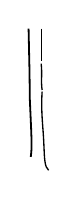
\begin{tikzpicture}[x=1mm,y=1mm]\draw[line width=.65pt] (0,18)--(.05,15.7)--(.12,12.5)--(.16,9)--(.32,5.4)..controls(.4,3.5)and(.4,2.5)..(.28,1.7);\draw[line width=.48pt] (1.6,18)--(1.6,13.85);\draw[line width=.48pt] (1.6,13.55)..controls(1.75,12.2)and(1.55,11.3)..(1.72,10.2);\draw[line width=.48pt] (1.72,10.0)..controls(1.55,7.3)and(1.85,5.7)..(1.95,3.1)..controls(2.02,1.6)and(2.02,.4)..(2.55,0);\end{tikzpicture}}}
(Demander à Quillen relations exactes entre \deleted{H}objets-groupes et objet
\inserted{\deleted{ponctués}}connexes de la catégorie homotopique\inserted{ponctuée}: forment-ils des catégories équival
tes par le foncteur espace des lacets\handwritten{?}).
\margin{\handwritten{non, on a\\un foncteur\\\unsure{pl.} fidèle (?)\\\unsure{mais} \unsure{pas} \unsure{ess.}\textsuperscript{t}\\surjectif....}}

Pour les \uline{vrais} groupes \inserted{abéliens} de (2-\unsure{\deleted{C}C|\deleted{o}C|\deleted{C}o}at), l'approche de Quillen consiste à
les identifier à'abord à des groupes abéliens de la catégorie \deleted{t}\handwritten{(}Bicat),
donc à des grpupes abéliens bi-semiesimpliciaux particuliers (conditions
sur chaque ligne et chaque colonne). Appliquant la version bi-semisimpli
ale du tapis de Dold, on trouve que \deleted{c\unsure{e}tt\unsure{e} c\unsure{a}} la catégorie de ces objets
esth équivalente à la catégorie des \deleted{objets} bicomplexes \inserted{de chaines} de groupes abéli
qui sont nuls en dehors du carré $\unsure{\deleted{D}0|\deleted{0}D}\handwritten{\leq}i,j\handwritten{\leq}1$. \deleted{Quillen dit que} La \deleted{colonn}\inserted{\handwritten{cond.}}
que la première ligne corresponde à un \deleted{ensemble} groupe semisimplicial
trivial signifie alors qu'elle n'a que le terme de degré zéro, i.e. que
le bicomplexe est réduit à

\diagram{
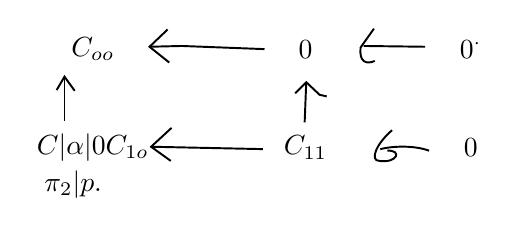
\begin{tikzpicture}[x=1cm,y=1cm,baseline=(current bounding box.center)]\node (a) at (0,1.25) {$C_{oo}$};\node (b) at (2.7,1.25) {$0$};\node (c) at (4.8,1.25) {$\handwritten{0}^{\unsure{\cdot}}$};\node (d) at (0,0) {$\handwritten{\unsure{C|\alpha|0}}C_{1o}$};\node (e) at (2.7,0) {$C_{11}$};\node (f) at (4.8,0) {$\handwritten{0}$};\node at (-.25,-.47) {$\unsure{\pi_{\unsure{2}}|p.}$};\draw[line width=.7pt] (2.18,1.25)--(1.13,1.29)--(.72,1.28);\draw[line width=.7pt] (.95,1.50)--(.72,1.28)--(.97,1.08);\draw[line width=.7pt] (4.22,1.28)--(3.44,1.29);\draw[line width=.7pt] (3.57,1.51)--(3.40,1.27)..controls(3.38,1.09)and(3.47,1.05)..(3.58,1.10);\draw[line width=.7pt] (2.16,-.02)--(.75,.01);\draw[line width=.7pt] (1.00,.25)--(.74,.01)--(.99,-.17);\draw[line width=.7pt] (4.27,-.04)..controls(4.08,.03)and(3.81,.02)..(3.65,-.02);\draw[line width=.7pt] (3.80,.22)..controls(3.60,.05)and(3.51,-.17)..(3.64,-.17)..controls(3.87,-.20)and(3.93,-.03)..(3.74,-.04);\draw[line width=.7pt] (-.36,.34)--(-.36,.90);\draw[line width=.7pt] (-.46,.73)--(-.36,.90)--(-.23,.72);\draw[line width=.7pt] (2.69,.32)--(2.71,.83);\draw[line width=.7pt] (2.57,.69)--(2.71,.83)--(2.88,.67)--(2.97,.65);\end{tikzpicture}
}
\margin{\handwritten{9}}
